\documentclass{article}

\usepackage{amsmath}
\usepackage{graphicx}
\usepackage{enumitem}
\usepackage{hyperref}

\title{4069 State Variable Filter}
\author{Guy John \\ \texttt{guy@rumblesan.com}}

\begin{document}

\maketitle

\section{Introduction}
The design for the Yorick filter was found on a \href{https://electro-music.com/forum/topic-69887.html}{thread on the the electro music forum}. A user called Hammer had created a filter based around the CD4069 CMOS inverter IC which could run off 5 volts, and give CV control of the cutoff. This document tries to run through the maths on how it works, and is mainly to try and help with figuring out the correct values for the design.

In the first version that Hammer shared they used JFETs as a variable resistance element to handle the voltage control, but specified the 2N5457 which is getting a bit pricy to get hold of, and isn't ideal if we want to keep things cheap. The J113 JFET should work reasonably well in it's place, but it's worth running through the maths to make sure, and see if and how we can improve things.

\newpage

\subsection{CMOS Inverter Linear Applications}

\subsubsection{Inverters as OpAmps}

The use of 4069 inverters as amplifiers isn't that uncommon, and it turns out that they can work pretty well. \href{https://www.modwiggler.com/forum/viewtopic.php?t=256633&hilit=4069+amplifier}{This thread on ModWiggler} has some really useful info on the subject, and famously the Wasp filter uses inverters as the integrators that are paired with the 3080 OTAs.

In terms of the analysis, we can assume that it will follow similar behaviour to an inverting op-amp circuit.

\begin{figure}[h]
  \caption{A CMOS inverter biased for linear mode operation, taken from the National Semiconductor Application Note 88 July 1973}
  \centering
  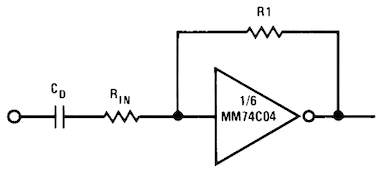
\includegraphics[width=\linewidth]{images/inverter-feedback-amplifier.png}
\end{figure}

Here the equation for the output voltage is $V_{out} = - V_{in} * \frac{R1}{R_{in}}$.

\subsubsection{Inverters as Integrators}

\begin{figure}[h]
  \caption{A CMOS inverter based integrator}
  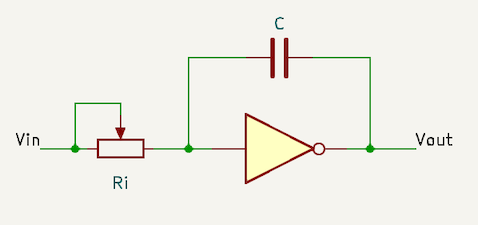
\includegraphics[width=\linewidth]{images/inverter-integrator.png}
\end{figure}

Knowing that the inverter works roughly the same as an inverting op-amp, we can also make the same assumption about how it works as an integrator.

Assuming that the input of the inverter self-biases to half the supply voltage, we can treat it as a virtual ground, meaning that the sum of all currents at that point should equal zero. This means that the current through the capacitor $C$ will be equal to the current flowing through $R_{i}$.

Working in the Laplace domain to make the analysis easier, we can state the following:

\begin{description}
\item $s$ is a complex frequency variable that can represent the phase and amplitude of a signal.
\item $v_{in}(s)$ is the input voltage in terms of $s$.
\item $R_{i}$ is the value of the resistor through which the input signal is fed to the integrator.
\item $C$ is the value of the integrators' capacitors.
\item $v_c(s)$ is the voltage across the capacitor in terms of $s$.
\item $i_c(s)$ is the current flowing into the capacitor in terms of $s$.
\end{description}

\begin{equation*}
\begin{split}
  v_c(s) & = \frac{i_c(s)}{Cs} \\
  i_c(s) & = \frac{v_{in}(s)}{R_{i}} \\
  v_{out}(s) & = -v_c(s) \\
             & = -\frac{i_c(s)}{Cs} \\
             & = -\frac{v_{in}(s)}{R_{i}}\frac{1}{Cs} \\
             & = -\frac{v_{in}(s)}{CsR_{i}} \\
  \frac{v_{out}(s)}{v_{in}(s)} & = -\frac{1}{CsR_{i}} \\
\end{split}
\end{equation*}

We can take the above equation and turn it into a transfer function $\alpha(s)$.

\begin{equation}
  \alpha(s) = -\frac{1}{CsR_{i}}
\end{equation}

\subsection{Filter Analysis}

\begin{figure}[h]
  \caption{The CMOS inverter based filter}
  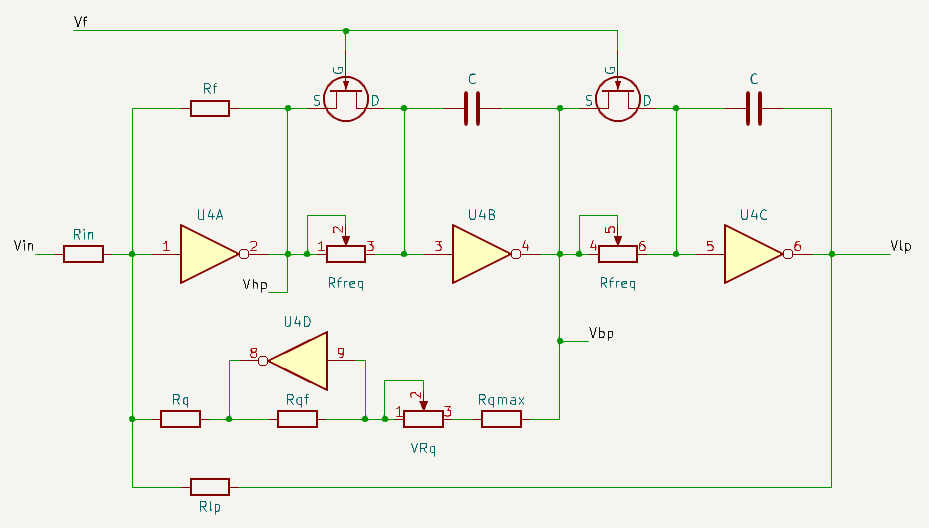
\includegraphics[width=\linewidth]{images/filter-circuit.png}
\end{figure}

For the time being we're going to ignore the JFETs and any affect that they might have on the circuit. Having them in parallel with the variable resistors means they can affect the overall resistance of the input to the two integrators and change the frequency response, but we can investigate their affect later.

The filter circuit actually gives us the high-pass, band-pass and low-pass signals as outputs, but we'll be primarily focussed on the low-pass signal here. It's still helpful to refer to these signals as $v_{hp}$, $v_{bp}$ and $v_{lp}$ though.

\subsubsection{Resonance Feedback Amplifier}

Inverter U4D along with resistors $Rq$, $Rqf$, $Rqmax$, and potentiometer $VR_q$ is responsible for the amount of band-pass signal getting fed back to the input, which controls the overall resonance. This is just an inverting amplifier with the potentiometer set to change the input resistance and so give manual control over the gain. The minimum gain will be $\frac{Rqf}{VRq + Rqmax}$, and the maximum gain will be $\frac{Rqf}{Rqmax}$, but these will be negative because the amplifier is inverting.

The setup with the potentiometer being used as a variable resistance instead of being tied to ground is because the bias point for the filter circuit is actually at $Vcc / 2$, but we would have to create this voltage as it doesn't currently exist in the circuit.

To simplify the equations for the time being, we'll just say this is a gain factor $-\beta$ which is controlled by the potentiometer rotation.

\subsubsection{Input Mixer}

The first stage of the filter is a summing mixer built around U4A.


\begin{equation}
  \frac{v_{in}(s)}{R_{in}} + \frac{v_{hp}(s)}{R_f} + \frac{v_{lp}(s)}{R_{lp}}  + \frac{{-\beta}v_{bp}(s)}{R_q} = 0
\end{equation}

It is useful to note that $v_{bp}(s) = v_{hp}(s)\alpha(s)$, and $v_{lp}(s) = v_{hp}(s)\alpha(s^2)$. Also to simplify here we'll set $R_{lp} == R_f$.

\subsubsection{High-pass}

\begin{equation*}
\begin{split}
  \frac{v_{hp}(s)}{R_{f}} & = - \frac{v_{in}(s)}{R_{in}} - \frac{v_{lp}(s)}{R_{f}} - \frac{v_{bp}(s)-\beta}{R_q} \\
  \frac{v_{hp}(s)}{R_{f}} & = - \frac{v_{in}(s)}{R_{in}} - \frac{v_{hp}(s)\alpha(s^2)}{R_{f}} - \frac{{-\beta}v_{hp}(s)\alpha(s)}{R_q} \\
  \frac{v_{in}(s)}{R_{in}} & = - \frac{v_{hp}(s)}{R_{f}} - \frac{v_{hp}(s)\alpha(s^2)}{R_{f}} - \frac{{-\beta}v_{hp}(s)\alpha(s)}{R_q} \\
  H_{hp}(s) & = \frac{v_{hp}(s)}{v_{in}(s)} \\
  \frac{v_{in}(s)}{R_{in}} & = - v_{hp}(s)(\frac{1}{R_{f}} + \frac{\alpha(s^2)}{R_{f}} + \frac{{-\beta}\alpha(s)}{R_q}) \\
  \frac{1}{R_{in}} & = - H_{hp}(s)(\frac{1}{R_{f}} + \frac{\alpha(s^2)}{R_{f}} + \frac{{-\beta}\alpha(s)}{R_q}) \\
  \frac{-1}{R_{in}} & = H_{hp}(s)(\frac{1}{R_{f}} + \frac{\alpha(s^2)}{R_{f}} + \frac{{-\beta}\alpha(s)}{R_q}) \\
  H_{hp}(s) & = \frac{-1/R_{in}}{\frac{1}{R_{f}} + \frac{\alpha(s^2)}{R_{f}} + \frac{{-\beta}\alpha(s)}{R_q}} \\
  & = \frac{-R_{f}/R_{in}}{1 + \frac{{-\beta}R_{f}\alpha(s)}{R_q} + \alpha(s^2) } \\
\end{split}
\end{equation*}

\subsubsection{Low-Pass}

\begin{equation*}
\begin{split}
  H_{lp}(s) & = \frac{v_{lp}(s)}{v_{in}(s)} \\
            & = \frac{v_{hp}(s)}{v_{in}(s)}\alpha^2(s) \\
            & = \frac{-R_{f}/R_{in}}{\frac{1}{\alpha^2(s)} + \frac{R_{f}-\beta}{R_q\alpha(s)} + 1 } \\
            & = \frac{-R_{f}/R_{in}}{\frac{1}{\alpha^2(s)} + -\beta\frac{R_{f}}{R_q}\frac{1}{\alpha(s)} + 1 } \\
            & = \frac{-R_{f}/R_{in}}{\frac{1}{{(-\frac{1}{CsR_{i}})}^2} + -\beta\frac{R_{f}}{R_q}\frac{1}{-\frac{1}{CsR_{i}}} + 1 } \\
            & = \frac{-R_{f}/R_{in}}{\frac{1}{{\frac{1}{(sCR_{i})^2}}} + \beta\frac{R_{f}}{R_q}\frac{1}{\frac{1}{sCR_{i}}} + 1 } \\
            & = \frac{-R_{f}/R_{in}}{s^2(CR_{i})^2 + \beta\frac{R_{f}}{R_q}sCR_{i} + 1 } \\
\end{split}
\end{equation*}

At this point we'll also make the simplification that $R_q = R_{f}$, giving the final transfer function for the low-pass output.

\begin{equation}
  H_{lp}(s) = \frac{-R_{f}/R_{in}}{s^2(CR_{i})^2 + \beta sCR_{i} + 1 } \\
\end{equation}

\subsubsection{Calculating Gain, Cutoff and Resonance}

For reference, the standard second-order filter transfer functions are:

\begin{equation*}
\begin{split}
  H_{lp}(s) & = \frac{1}{s^2T^2 + \frac{1}{q}sT + 1} \\
  H_{bp}(s) & = \frac{1}{\frac{q}{sT} + qsT + 1} \\
  H_{hp}(s) & = \frac{1}{\frac{1}{s^2T^2} + \frac{1}{qsT} + 1} \\
\end{split}
\end{equation*}

By comparing our transfer function with the standard one for a low-pass, we can work out the following.

\begin{description}
  \item Pass-band gain, $-\frac{R_{f}}{R_{in}}$
  \item Cutoff frequency, $\frac{1}{2{\pi}T} \rightarrow x\frac{1}{2{\pi}CR_{i}}$
  \item Resonance, $\frac{1}{\beta}$
\end{description}

\subsection{Calculating Cutoff Frequencies}

Given the calculation for frequency, and picking some standard values we can calculate cutoff for different $i_{cv}$ values.

\begin{description}
  \item $R_i$ is between 47r and 10k
  \item $C$ is 220nF
\end{description}

\begin{equation}
  f = \frac{1}{2{\pi}CR_i}
\end{equation}

\begin{description}
  \item for $R_i$ of 47r  $f = 15395Hz$
  \item for $R_i$ of 1k   $f = 723Hz$
  \item for $R_i$ of 5k   $f = 145Hz$
  \item for $R_i$ of 10k  $f = 72Hz$
\end{description}

\subsection{Calculating Resonance}

The resonance here is directly proportional to the gain of the resonance feedback stage, with lower gains meaining higher resonances. A resonance value of around 0.5 is a good minimum, with higher values being more resonant.

\begin{equation*}
\begin{split}
  \beta & = \frac{R_{qf}}{VR_q + R_{qmin}} \\
  res   & = \frac{1}{\beta} \\
  res   & = \frac{VR_q + R_{qmin}}{R_{qf}} \\
  {\min res} & = \frac{R_{qmin}}{R_{qf}} \\
  {\max res} & = \frac{VR_q + R_{qmin}}{R_{qf}} \\
\end{split}
\end{equation*}


\subsubsection{Actual Values}

In our final design, $VR_{q}$ is 100k, $R_{qf}$ is 10k, and $R_{qmin}$ is 4k7, giving a final resonance range of,

\begin{equation*}
\begin{split}
  {\max res} & = \frac{VR_{q} + R_{qmin}}{R_{qf}} \\
             & = \frac{100k + 4k7}{10k} \\
             & = 10.47 \\
  {\min res} & = \frac{R_{qmax}}{R_{qf}} \\
             & = \frac{4k7}{10k} \\
             & = 0.47 \\
\end{split}
\end{equation*}


\end{document}
